\section{\label{sec:intro}Introduction\protect}
The scattering of pions off of atomic nuclei has been the subject of extensive study
%, particularly during the second half of the 20th century,
due to its ability to serve as a probe of the nuclear structure 
%in the context of effective theories
through the understanding of the interactions among mesons and nucleons. The $\Delta(1232)$ pion-nucleon resonance dominates in the sub-GeV energy region, and thus the range of $p_{\pi}$ between 200 to 300 MeV$/c$ is of special interest.

%In the case of $\pi^{\pm}-$C interactions this corresponds to $p_{\pi}$ in the 200 to 300 MeV$/c$ range.

The dominant $\pi^{\pm}$-A interactions in the sub-GeV region are represented diagrammatically in Fig. \ref{fig:interactions}. The total, elastic and quasi-elastic processes have been measured with $<10\%$ precision by various experiments \cite{Allardyce,Binon,Saunders,Gelderloos,Levenson,Ashery2,Ingram,Jones,Ashery,Bellotti1973,Bellotti1973_2}, however data are scarce for inelastic processes such as absorption (ABS: $\pi^{\pm}+A\rightarrow (A-N) + N$) and single charge exchange (CX: $\pi^{\pm} + A \rightarrow \pi^{0}+ (A-N) + N$), where ``N" represents any number of nucleons leaving the nucleus. Moreover, the majority of past experiments measured the combined rate of these two processes \cite{gianneli,navon}, and relied on other experimental results or on theoretical calculations to separate their individual contribution while ignoring possible correlations and systematic uncertainties.

\begin{figure}[ht]
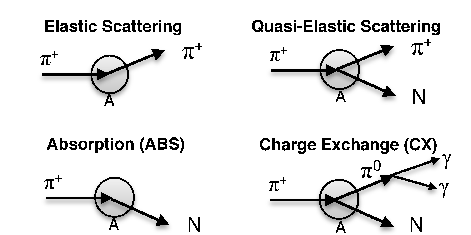
\includegraphics[width=86mm]{figures/Figure1_sep_paper_b_w.eps}
\caption{Dominant $\pi^{\pm}$-A interactions in the sub-GeV region. ``N" represents any number of nucleons leaving the nucleus.}
\label{fig:interactions}
\end{figure}

Interest in pion inelastic interactions has increased in recent years due to the use of nuclear targets in GeV-scale neutrino experiments. Neutrinos are primarily detected via charged-current quasi-elastic interactions ($\nu_{\mu}+n\rightarrow \mu^{-} + p$) with target atomic nuclei. The neutrino-induced single pion production processes also contribute to the cross section in this energy range. The energy of the neutrino is fundamental to probing the oscillation phenomena and is inferred from the measured kinematics of the outgoing lepton.  If the pion is produced but not detected due to final-state interactions (FSI) within the target nucleus or secondary interactions (SI) elsewhere in the detectors, the inferred neutrino energy will be biased. 

FSI and SI are leading contributors to systematic uncertainties in neutrino oscillation and cross section experiments. Their impact is typically evaluated using predictions based on models implemented in Monte Carlo neutrino event generators such as \textsc{Neut} \cite{NEUT} and \textsc{NuWro} \cite{NuWro} for FSI, or detector simulation toolkits such as \textsc{Geant4} \cite{bertini} and \textsc{Fluka} \cite{fluka1,fluka2} for SI. Some of these generators use similar implementations of semi-classical cascade models in which the pion is propagated within the nucleus and its fate is calculated following theoretical optical models in which the pion-nucleus scattering is represented as a wave in a complex potential. The real part of the potential is responsible for elastic scattering while the imaginary part gives the contributions from inelastic channels \cite{Oset,Salcedo}. Precise tuning of the models is achieved through the empirical scaling of the theoretical microscopic interaction rates, relying entirely on the available $\pi^{\pm}$-A scattering data. Other important scenarios in which $\pi^{\pm}$-A interactions are relevant for neutrino physics are: i) the enhancement of the neutral-current $\pi^{0}$ background in neutrino oscillation appearance experiments, and, ii) pion reconstruction capabilities in water Cherenkov detectors via the explicit identification of their hadronic interactions.

An earlier paper from the DUET Collaboration \cite{duet} described our experimental setup and presented a measurement of the combined ABS and CX cross section $\sigma_{\mathrm{ABS}+\mathrm{CX}}$ in the 200 to 300 MeV$/c$ region. In this paper, we present separate measurements of $\sigma_{\mathrm{CX}}$ and $\sigma_{\mathrm{ABS}}$ for various momenta. This was achieved by extending the selection using a downstream detector to tag forward-going photons from the decay of a $\pi^0$ produced in a CX interaction. This measurement will help improve the modeling of FSI and SI and to reduce the associated systematic uncertainties on current and future neutrino oscillation and cross section experiments.